\documentclass[a4paper]{article}
\usepackage[margin = 1 in]{geometry}
\usepackage{fancyhdr}
\usepackage{lastpage}
\usepackage{ctex}
\usepackage[utf8]{inputenc} % Required for inputting international characters
\usepackage[T1]{fontenc} % Output font encoding for international characters
\usepackage[sfdefault]{ClearSans} % Use the Clear Sans font (sans serif)
\usepackage{tocloft} 
\usepackage{makecell}%导入表格宏包
\usepackage{bmpsize}
\usepackage{graphicx}
\usepackage{epstopdf}
\usepackage{caption}
\usepackage{enumitem}
\usepackage{float}
\usepackage{multirow}
\usepackage{makecell}
\usepackage{wrapfig}
\usepackage{tcolorbox}
\usepackage[hidelinks]{hyperref}
\usepackage{xcolor}

\pagestyle{fancy}
\lhead{\textsl{\href{https://team23-22.bham.team}{\textcolor{blue}{App description}}}}
\chead{}
\rhead{Page \thepage\ of \pageref{LastPage}}
\lfoot{}
\rfoot{}
\cfoot{}
\renewcommand{\headrulewidth}{0.4pt}
\renewcommand{\footrulewidth}{0pt}
\renewcommand{\cftsecleader}{\cftdotfill{\cftdotsep}}
\newcommand{\tabincell}[2]{\begin{tabular}{@{}#1@{}}#2\end{tabular}} %单元格内换行

\renewcommand*\contentsname{Table of Contents}

\begin{document}

%----------------------------------------------------------------------------------------
%	TITLE PAGE
%----------------------------------------------------------------------------------------

\begin{titlepage}
	
	\rule{\linewidth}{5pt}
	\raggedleft
	\fontsize{38pt}{50pt}\selectfont
    \textbf{\\Team Project\\}
    \fontsize{28pt}{60pt}\selectfont 
    for\\
    \fontsize{38pt}{60pt}\selectfont 
    \textbf{App description\\}
	
	\vfill % Space between the title box and author information
	
	%------------------------------------------------
	%	Author name and information
	%------------------------------------------------
	
	\parbox[t]{0.93\textwidth}{ % Box to inset this section slightly
		\raggedleft % Right align the text
		\large % Increase the font size
		{\Large By Team 23-22}\\[4pt] % Extra space after name
		Bogdan-Marian Gheorghe\_2329324\_bxg125\\
		Chance Egbon\_2194210\_cee010\\
		Gilead Bempah\_2296232\_gxb035\\
		Matthew Goulding\_2330080\_mxg183\\
		Samuel Okasia\_2345883\_sxo183\\
		Smit Navinkumar\_2327596\_sxn197\\
		Zijun Li\_2272583\_zxl183\\
	}
	
\end{titlepage}

\section*{App Description}

The Time Management web application offers a user-centric and highly accessible experience through its intuitive web front end, compatible with standard browsers. Designed to optimize productivity, the application enables users to manage their time effectively by organizing tasks, setting reminders, and visualizing their schedule with ease. The responsive design ensures a seamless experience across various devices, while the clean layout and straightforward navigation allow users to effortlessly access all essential functions.

Comprising seven powerful features - Scheduler, Todo-List, Anti-Procrastination, Alarm, Diary, Email Notifications, and History - the application is specifically tailored to help users gain control over their time management. This comprehensive solution empowers users to achieve their goals and make the most of their time.

Todo List is a very daily and brief function. Users can add to-do items, and then click the circle in front to switch to done items whenever they are finished. At the same time, click on the name of a to-do item to display its detail window. Each item can be edited in detail, and the user can modify the heading and description to help memorize the to-do item. At the same time, the creation time and last modification time of each to-do item will be recorded. The interface is simple, the windows can be opened and closed smoothly, and the simplest functions are used to give users the most comfortable experience.

\begin{figure}[H]
    \centering
    \begin{minipage}{0.49\textwidth}
      \centering
      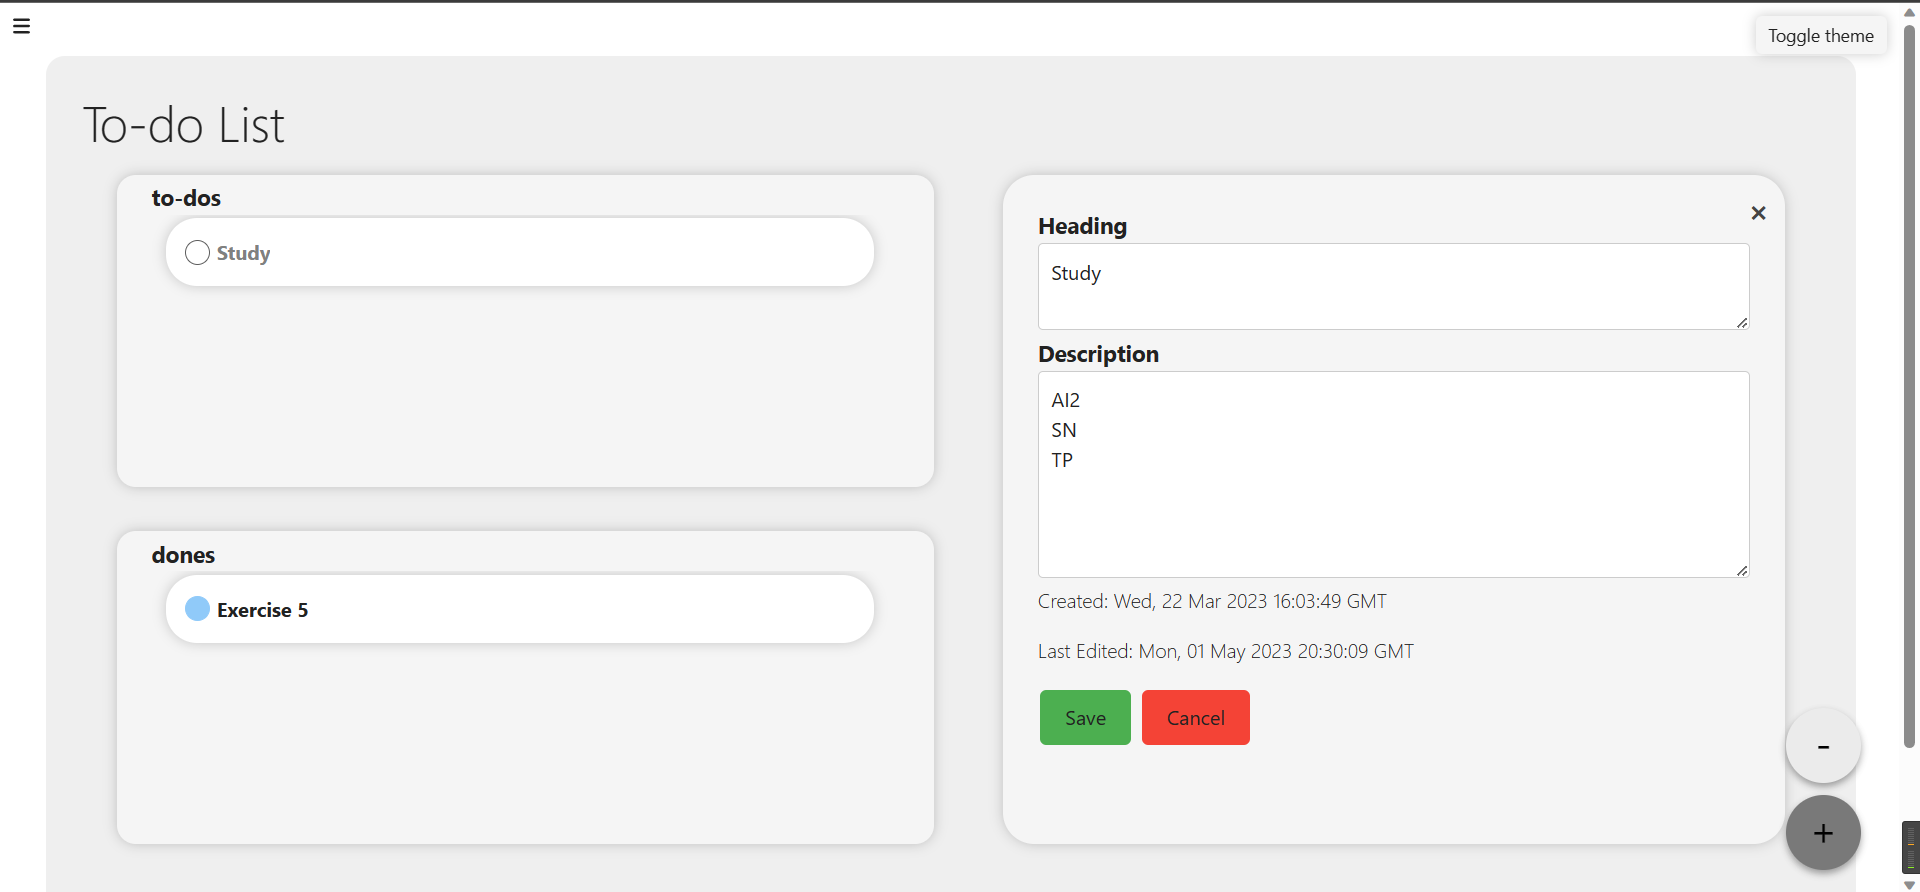
\includegraphics[width=\linewidth]{./image/Todo_list_light.png}
    \end{minipage}\hfill
    \begin{minipage}{0.49\textwidth}
      \centering
      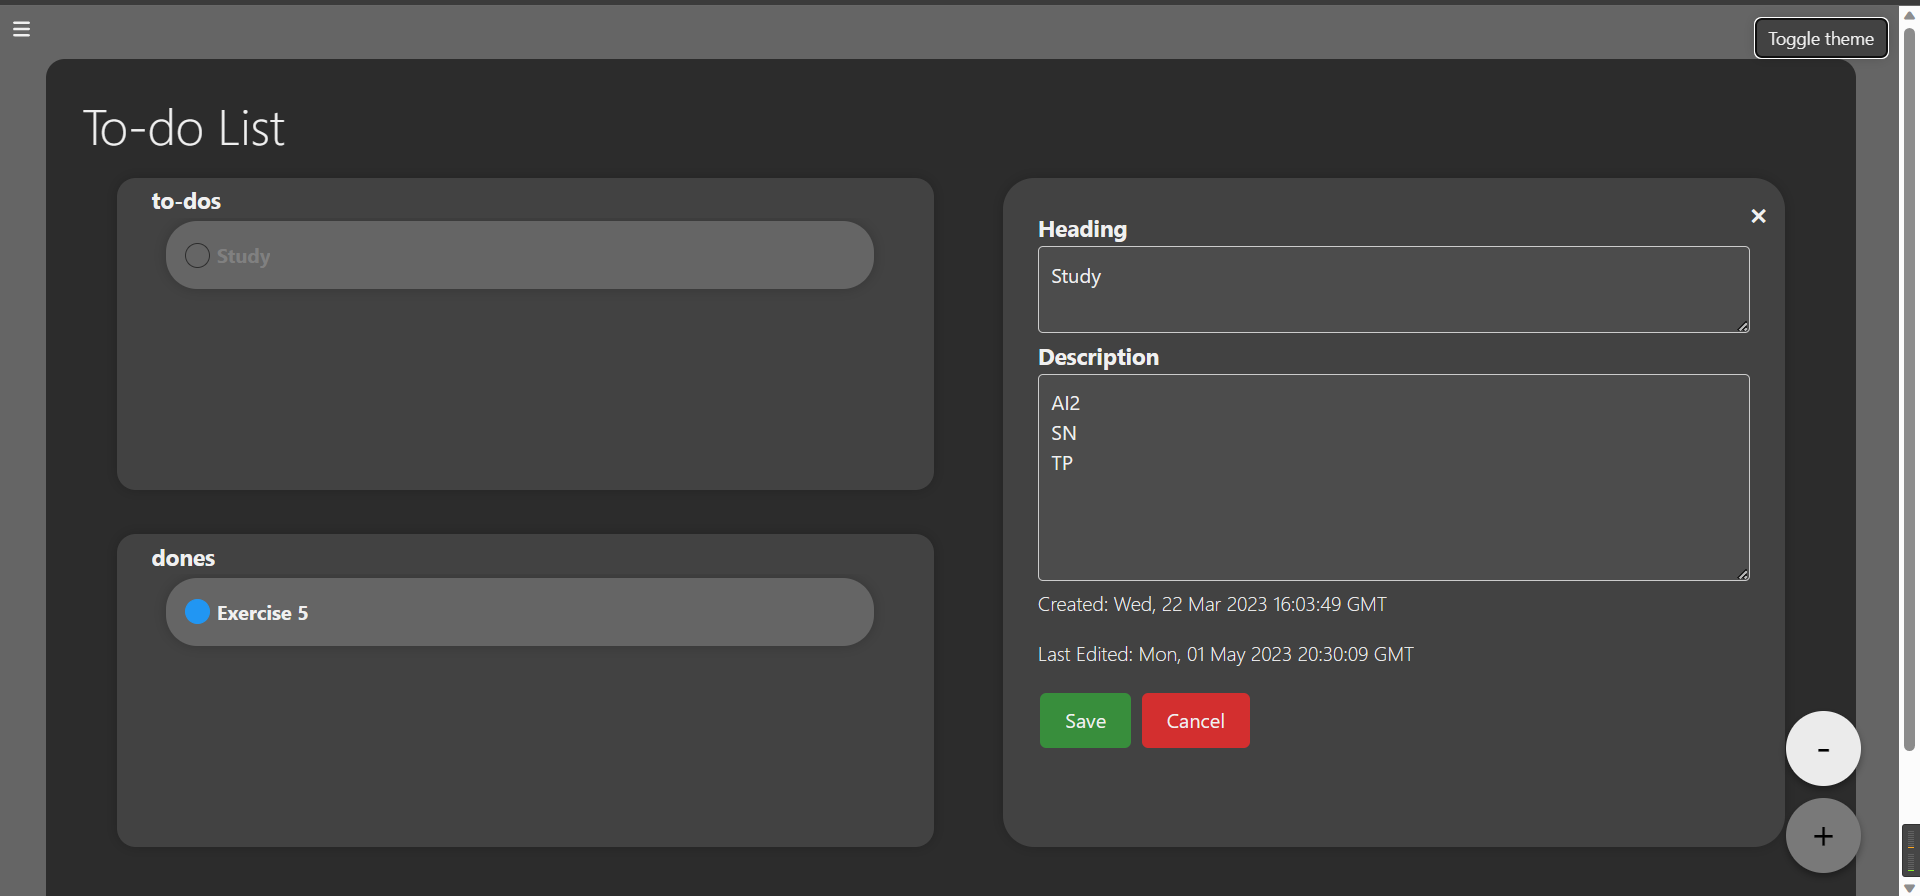
\includegraphics[width=\linewidth]{./image/Todo_list_dark.png}
    \end{minipage}
\end{figure}

Users can choose whether they want these website restrictions to be temporary or permanent via the Anti Procrastination feature, which enables users to block websites they may find distracting in order to help them focus on their work.
Whenever a user tries to access a site on their blocked list, the HTML of the
website will be replaced with the HTML present in the Content.js of the Chrome extension.
When a user returns to the Procrast website, the timers reset themselves, which means that they continue to count down even after the user departs.
The user can decide if they want to remove a block easily by just clicking a button next to the link allowing them to access that website again.

The User can visualise currently active blocks by just clicking on the Chrome extension,  which will display the Users Extension ID required in order for the extension to work and the blocked websites the user currently has.
The Anti Procrastination feature is unfortunately only exclusive to Google Chrome users

\begin{figure}[H]
    \centering
    \begin{minipage}{0.49\textwidth}
      \centering
      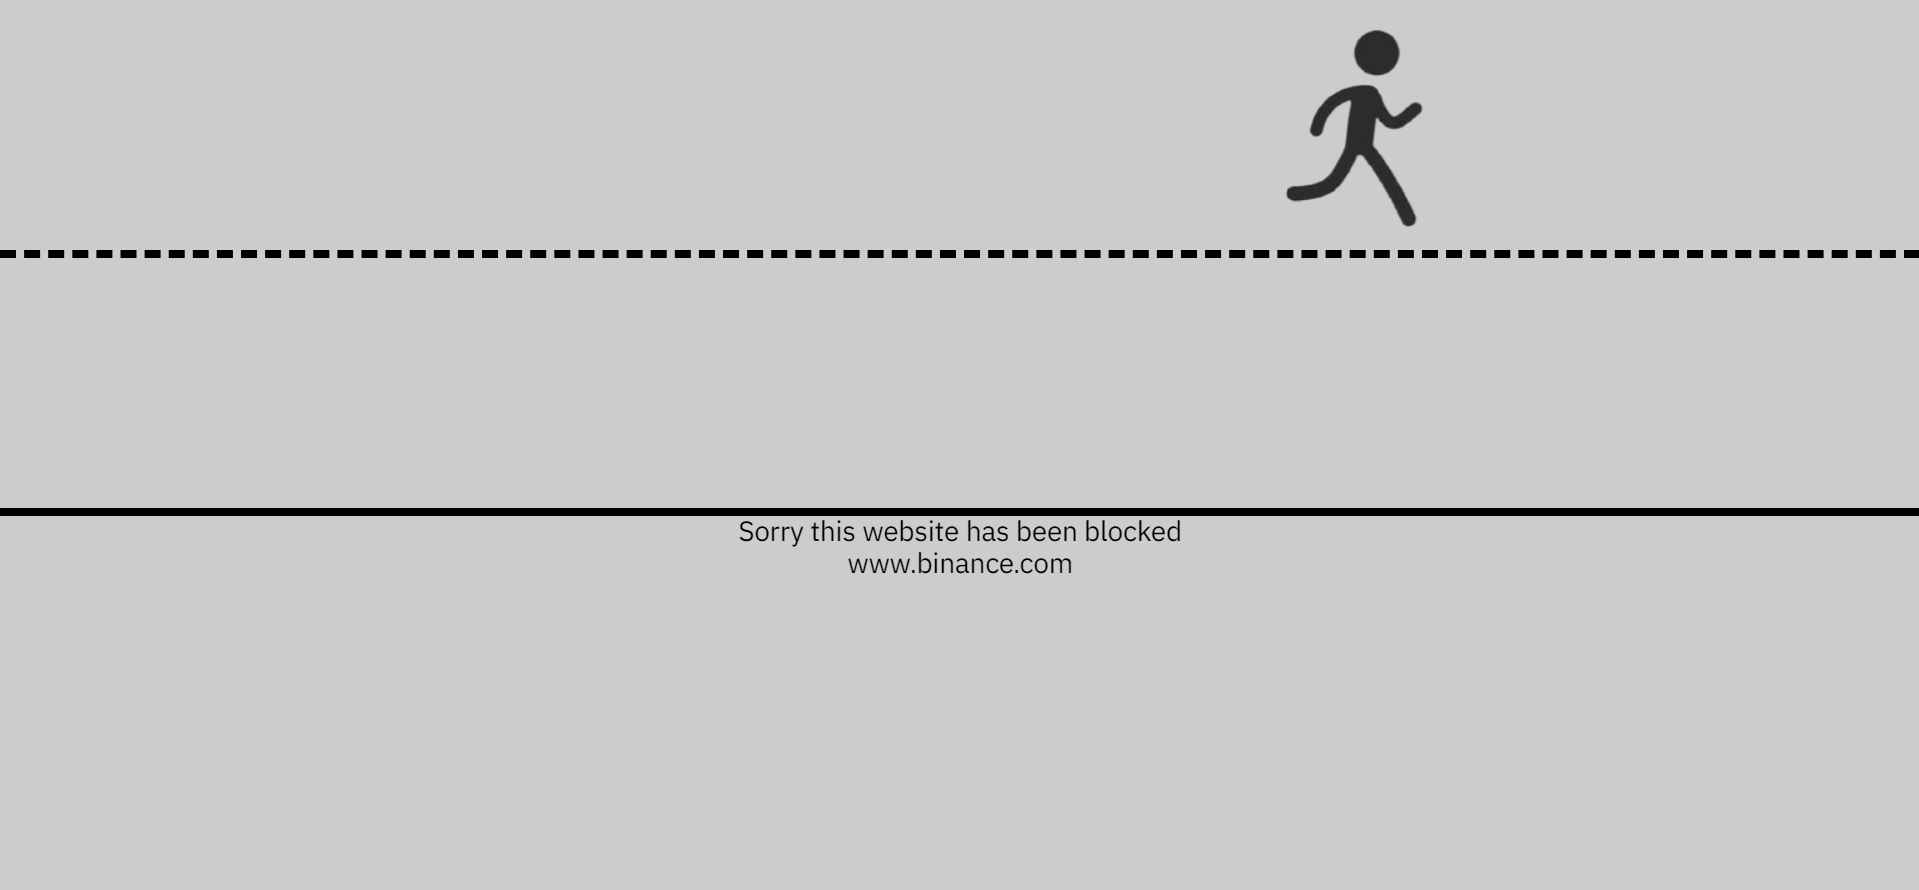
\includegraphics[width=\linewidth]{./image/BlockedWebsite.png}
    \end{minipage}\hfill
    \begin{minipage}{0.49\textwidth}
      \centering
      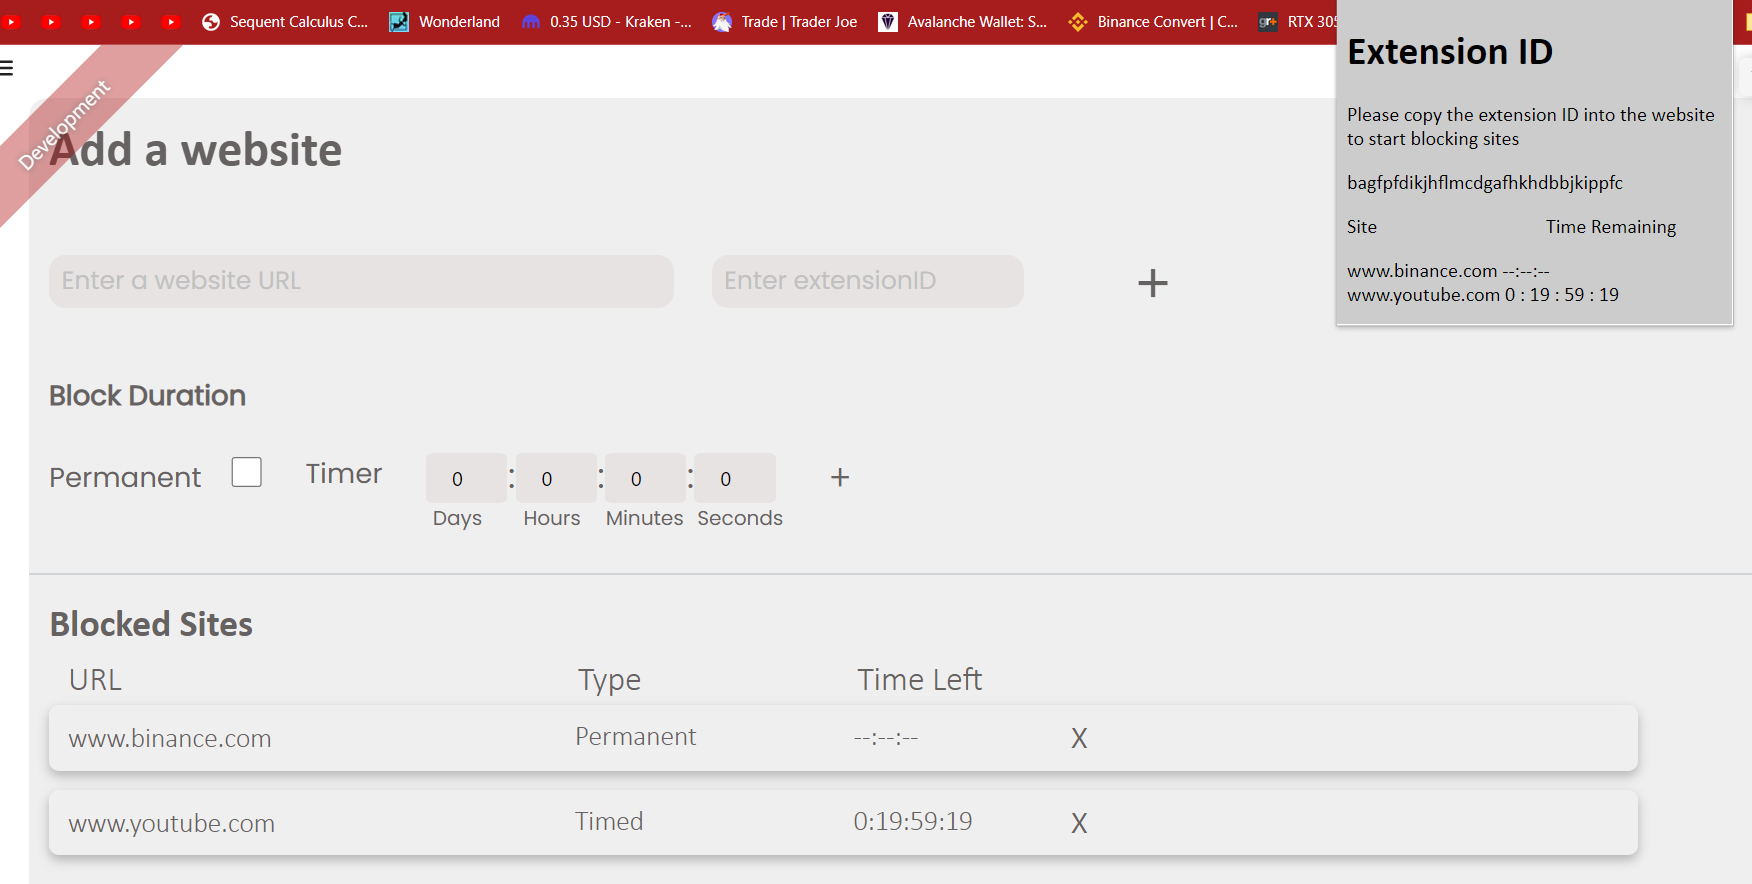
\includegraphics[width=\linewidth]{./image/AntiProcr.png}
    \end{minipage}
\end{figure}

The alarm/timer feature provides users with a tool to manage their time and stay focused on their tasks. The user is greeted with a user-friendly interface that allows them to easily add alarms or timers based on their needs. When adding an alarm or timer, users can specify the alarm name, choose between an alarm or timer type (which determines whether it counts up or down), and set the desired time. The alarms and timers are used by the user to stay focused on their tasks and therefore increase their productivity.

The history page is modern and user friendly function and is designed to help users keep track of their test scores and targets,. The graph allows users to visualize their progress over time,  by allowing them to add their own test subject and corresponding test scores to the graph. Users can also add their upcoming test and targets and then see their target scores for upcoming tests on dedicated display, helping them stay focused on where they need to improve.

\newpage
{\noindent\begin{tabular}{|p{0.25\linewidth}|p{0.70\linewidth}|} 
	\hline
 \textbf{Basic level of sophistication} & \textbf{Description} \\
 \hline
 Have a web front end accessible from a standard browser & The Time Management app features a user-friendly interface, accessible via standard browsers, ensuring seamless interaction across devices and easy access to essential functions.\\
 \hline
 Store some user-specific state in a database&  All the data includes both user and administrator are stored in the mysql database in the provided VM\\
 \hline
 Include a relevant GDPR privacy policy for all personal information & The GDPR privacy policy is shown in \href{https://team23-22.bham.team/GDPR-policy&DPIAForm}{\textcolor{blue}{https://team23-22.bham.team/GDPR-policy\&DPIAForm}}\\
 \hline
 Use the given git repository for version control - team members must submit their own code via their own user account&  The team employs the provided git repository for version control, ensuring each member submits code via individual accounts, promoting collaboration and streamlined development. The domain of the gitlab repository is \href{https://git.cs.bham.ac.uk/team-projects-2022-23/team23-22}{\textcolor{blue}{https://git.cs.bham.ac.uk/team-projects-2022-23/team23-22}}\\
 \hline
 Use a CI/CD pipeline - we have provided an example pipeline and skeleton app&  The app utilizes a CI/CD pipeline, automating the integration and deployment process, resulting in faster, more reliable releases and easier maintenance. 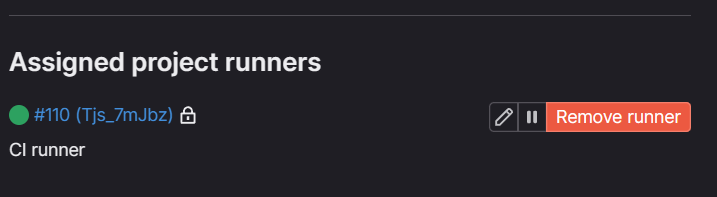
\includegraphics[width=10cm]{./image/CI_CD.png}\\
 \hline
 The app should be deployed and accessible publicly - we have provided a VM for this purpose& The app is deployed on a provided VM(amazon-VM), allowing public access, ensuring users can conveniently access the platform's features from any location.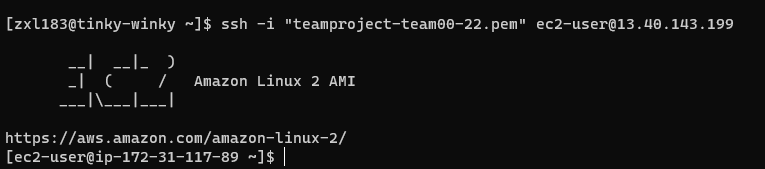
\includegraphics[width=9cm]{./image/VM.png}\\
 \hline
 Use a domain https:// (encrypted) and disallow http:// (plain text) requests &  The app employs HTTPS to encrypt data transmission, enhancing security and privacy, while disallowing plain-text HTTP requests to prevent data breaches. The domain is \href{https://team23-22.bham.team}{\textcolor{blue}{https://team23-22.bham.team}}\\
 \hline
 Implement features using “vertical slicing” & Features are developed using vertical slicing, allowing end-to-end functionality for each feature(frontend, backend and database), streamlining the development process and facilitating incremental improvements. 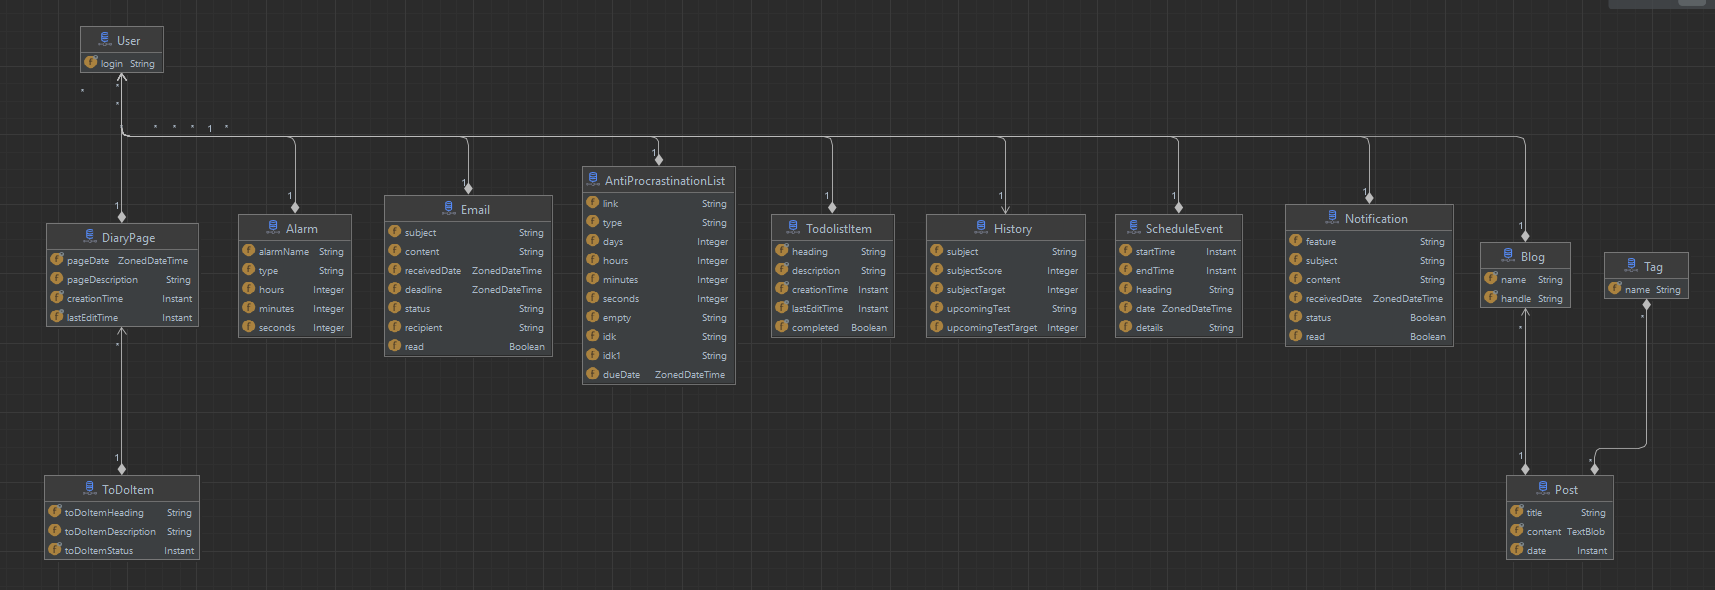
\includegraphics[width=10cm]{./image/Vertical_slice.png}\\
 \hline
\end{tabular}}

\newpage
{\noindent\begin{tabular}{|p{0.25\linewidth}|p{0.75\linewidth}|}
\hline
\textbf{Advanced Sophistication} & \textbf{Description} \\
\hline
Use complex APIs or libraries to implement useful features & In order to block websites, our application uses a Chrome extension. This extension has an external message listener that checks to see if any new websites have been added to or removed from the blocked list in the feature. When we add a new website, we send the link as a string to the extension, which then uses the Chrome Storage API to store or remove the website from the user's Chrome local storage.
The website https://.. is checked to see whether it matches one of the strings whenever a user enters a new site; if it does, the document's body is changed with the one from the Content.js file. \\
\hline
Integrate with existing systems or services & In our feature, we created a line graph using Chart.js, TypeScript, HTML, and CSS to display test subjects and their corresponding grades. We began by importing the Chart.js library and arranging my data as an array of objects with the topic name and the appropriate grade. We then built a new instance of the Chart object using JavaScript, supplying the canvas element and the data as parameters. We completed this after adding a canvas element to the HTML file. After that, We customised the chart's title, legend, and axes. Finally, We utilised CSS to embellish the chart as needed. The end result was a graph that was both aesthetically beautiful and instructive and effectively highlighted the relationship between test subjects and grades. \\
\hline
% \end{tabular}}
% 
% {\noindent\begin{tabular}{|p{0.25\linewidth}|p{0.75\linewidth}|}
% 	\hline
% 	\textbf{Advanced Sophistication} & \textbf{Description} \\
% \hline
Demonstrate creativity and flair in the features implemented & In addition to basic time management features like a scheduler and to-do list, the app includes an anti-procrastination feature that blocks distracting websites, ensuring user focus. \\
\hline
Look aesthetically pleasing, with a clear visual identity and relevant URL & The app features a clean, sleek design with smooth transition animations for a comfortable user experience. It also includes a dark mode for use in low-light environments. \\
\hline
\end{tabular}}

\end{document}